\hfill

\section{Multi-Player Quantum Games}
From the previous analysis done, it became clear that moving from a classical to a quantum game corresponds to a huge increment of the set of available strategies: just considering 2-players games as above, the number of possibilities accessible to both players moved from 2 to basically infinite. And the same consequence could hold also for the number of equilibria of the match, making the computational analysis very challenging.\\
For this reason, the extension of the previous formulation to games with more than two players will be very difficult but, at the same time, will provide new and surprising results. One of the first and most complete attempts is traceable to Benjamin and Hayden \cite{Benjamin_2001} in 2001 that, via the formulation and successive analysis of famous multi-player games like the Prisoners' Dilemma and the Minority Game, have shown that, differently from classical problems, several quantum players are able to cooperate to perfectly exploit their environment and guarantee the highest payoff to anyone. And the key ingredient that gives rise to this possibility is the entanglement among the different players' states.\\
\begin{figure}[t]
	\centering
	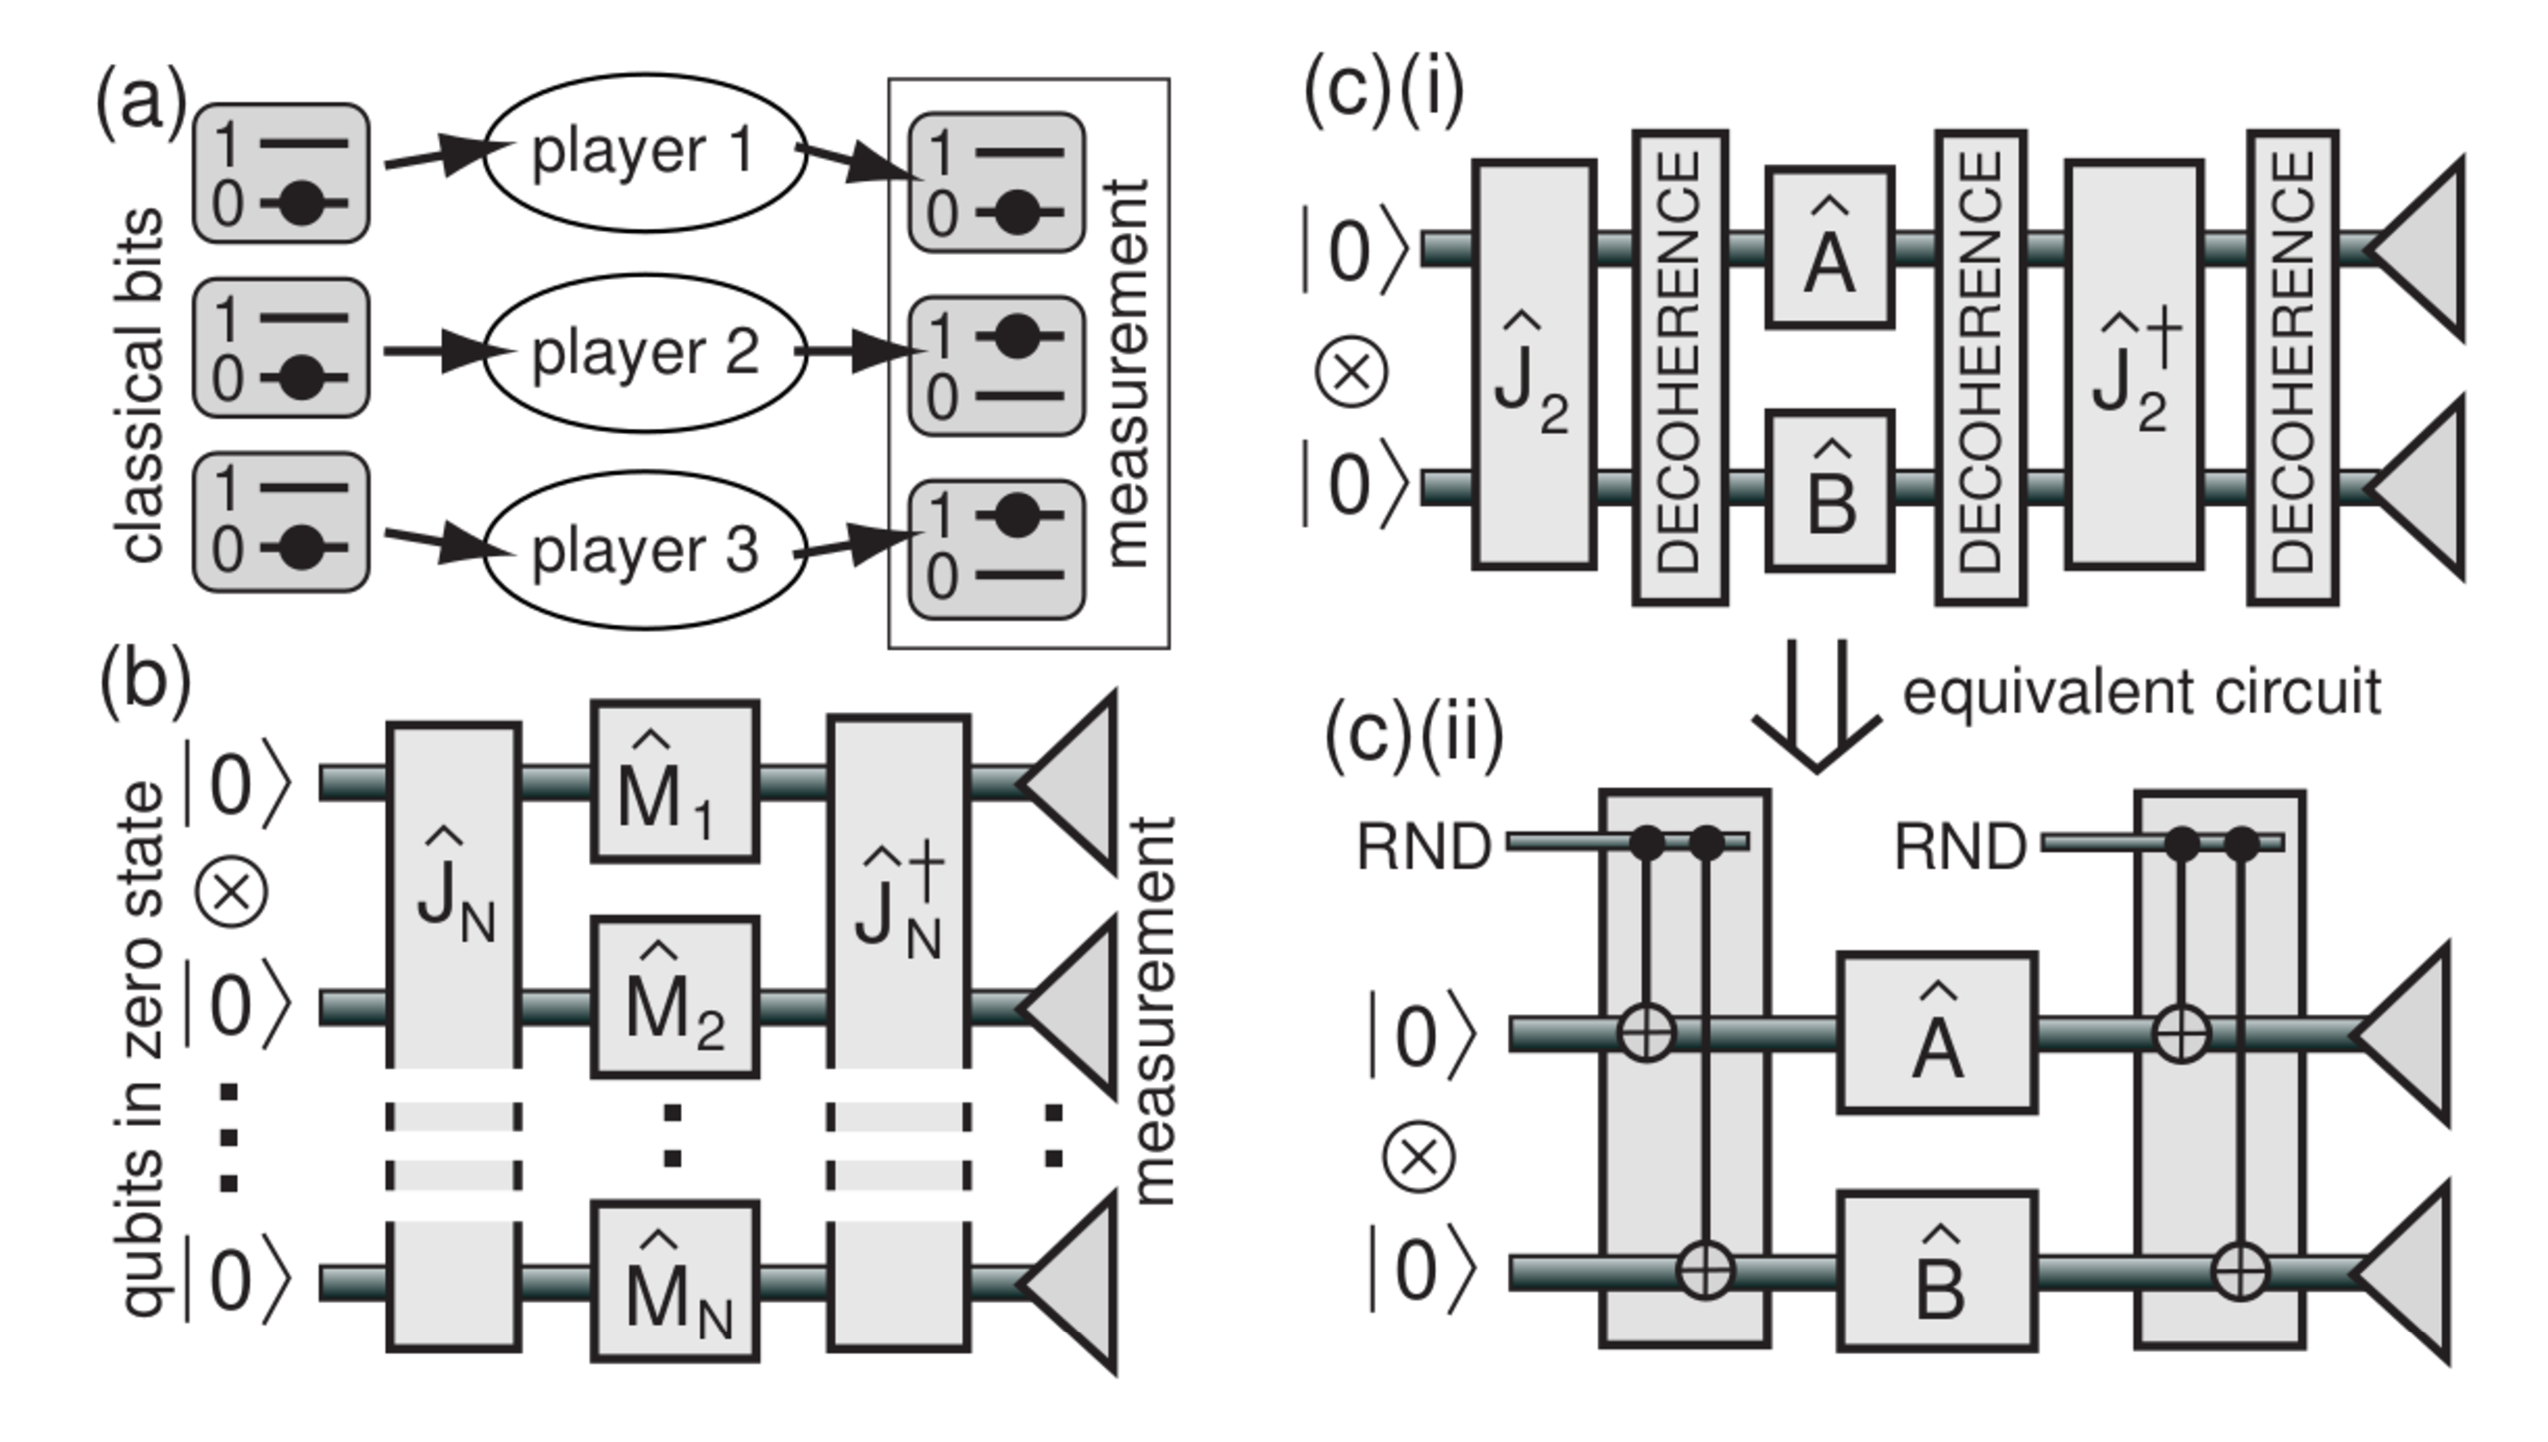
\includegraphics[scale=0.2]{pictures/multiplayer.pdf}
	\caption{(a) classical game in which each player has two actions available (flip or not) and the state of the system is a set of bits. (b) an N-player quantized game. (c) a more "realistic" version of the quantized game in which also the decoherence (progressive lost of quantum correlations) is took into account.}
	\label{fig:multi}
\end{figure}
The formulation suggested by Benjamin and Hayden, reported in figure \ref{fig:multi} is a generalization of the elegant scheme proposed also by Eisert \cite{Eisert_2020} in which: 
\begin{itemize}[noitemsep]
\item[-] each player is associated to a qubit, and all the qubits together represent a state of the system;
\item[-] such qubits can be entangled;
\item[-] the pure strategies available to the players are single-qubit operators represented by maps that are unitary, trace-preserving and positive defined;
\item[-] it should be possible to re-derive the classical game as a particular case.
\end{itemize}
Regarding the third point of the list, someone could argue about the fact that in classical games, the only restrictions over the action space were those imposed by classical physics: well, formally one could build a quantum game leaving players to choose among all the possibilities offered by the entire quantum mechanics, but he would end up with a problem nearly impossible to analyze, simulate or implement, and probably without any practical application.\\
To avoid making this paper too much long, the analysis of the 3-Prisoners' Dilemma and the N-player Minority Game will not be reported: the only thing that is worth to recall is that, as anticipated, entanglement acts as a sort of "contract" among the different contenders, that allows them to play "cooperatively" knowing that no one can successfully "defect" against the others.\\
Apparently, in the last years, you cannot find any other work like the one of Benjamin and Hayden, or at least of the same relevance, focused on the theoretical formulation of Multi-Player Quantum Games. The reason is probably mainly the difficulty of the analysis: redefining the problem in a quantum world means basically moving from a discrete to a continuous set of possibilities, with a consequent infinite number of different situations. Also simulating an N-player problem on a classical computer is almost impossible, as long as you want to obtain results with a reasonable accuracy.